\documentclass{article}
\usepackage[letterpaper]{geometry}
\geometry{verbose,tmargin=1in,bmargin=1in,lmargin=1in,rmargin=1in}

\usepackage[utf8]{inputenc}
\usepackage{amsmath}
\usepackage{listings}
\usepackage{graphicx}
\usepackage{enumitem}

\title{CIS 419/519: Homework 2}
\author{\{Yupeng Li\}}
\date{}

\begin{document}
    \maketitle
    Although the solutions are entirely my own, I consulted with the following people and sources while working on this homework:
     \{http://www.cs.utep.edu/vladik/cs5315.13/cs5315\_13kader.pdf\}
    
    \section{Gradient Descent}
    
    Let k be a counter for the iterations of gradient descent, and let $\alpha_{k}$ be the learning rate for the $k^{th}$ step of gradient descent.\\
    
    
a.) In one sentence, what are the implications of using a constant value for $\alpha_R{k}$ in gradient descent?


The $\alpha_{k}$ used is already the optimum value which will help converge $\theta_{j}$ to the minimum at quick enough speed 


b.) In another sentence, what are the implications for setting $\alpha_{k}$ as a function of k?

We have not yet decided the optimum $\alpha_k$ for convergence, thus we are checking if $\alpha_k$ is too big or too small



    
    
    \section{Linear Regression}
Since as we know the defined X has a Gaussian with mean 0 and variance, we can confidently assume
\[\frac{\partial}{\partial \theta}\mathcal{L}(\theta) = 0 \]

Thus we can safely use the closed form solution:
\[\theta =  (X^{T} X)^{-1} X^{T} y\]

Using this $\theta$ we can get from the following equation:

\[h_{\theta}(x_{i}) = x_{i}^{T} \theta\]

So that:

\[h_{\theta}(x) = \sum_{i=1}^{n}  x_{i}^{T} \theta\]
\[h_{\theta}(x) = \sum_{i=1}^{n}  x_{i}^{T} (X^{T} X)^{-1} X^{T} y_{i}\]
\[h_{\theta}(x) = x^{T} (X^{T} X)^{-1} X^{T} y\]

Where as we can see, X^{T} X)^{-1} X^{T} is a linear function of (X;x)

So that we can express that :

\[h_{\theta}(x) = x^{T} (X^{T} X)^{-1} X^{T} y\]

in the other way:

\[f(x) = \sum_{i=1}^{n} l_i(x;X)y_{i}\], where\[l_i(x;X)y_{i} = x_{i}^{T} (X^{T} X)^{-1} X^{T} y_{i}  \]

Obviously, \[(X^{T} X)^{-1} X^{T}\] is a a linear function that does not depend on y_{i}

	\section{Polynomial Regression}
		\subsection{Implementating Polynomial Regression}
This section is submitted in a separate .py file.

		\subsection{Choosing the optimal \lambda}

				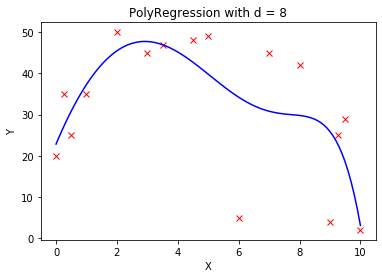
\includegraphics[width=\linewidth]{Unregularized.png}
				\caption{Unregularized graph with \lambda = 0}
 		
	
				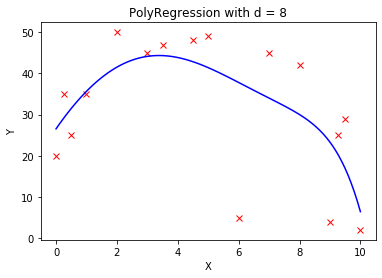
\includegraphics[width=\linewidth]{Regularized.png}
				\caption{Regularized graph with \lambda = 0.01}

One thing interesting is that, using the $\alpha$ given such that $\alpha$ = 0.25, the polynomial fitting does not converge when $\lambda$$ is 0.

Because of that, I tuned $\alpha$ to 0.01 so that the graph both converges at $\lambda = 0$ and $\lambda$ greater than 0.

The graphs are provided as above.



        
\end{document}